\documentclass[11pt,a4paper]{article}

\usepackage[margin=2.5cm]{geometry}
\usepackage{fontspec}
\setmainfont{TeX Gyre Termes}
\usepackage{tikz}
\usetikzlibrary{positioning, calc}
\usepackage[hidelinks]{hyperref}
\usepackage{titlesec}
\titleformat{\section}{\large\bfseries}{\thesection}{1em}{}
\titlespacing*{\section}{0pt}{2ex plus .5ex}{1ex}

\setlength{\parindent}{0pt}
\setlength{\parskip}{0.5ex}

\begin{document}

\begin{center}
  {\LARGE\bfseries Assignment 004: Personal Diary}\\[0.6ex]
  {\large Program Report}\\[0.6ex]
  Zheng Yifeng \quad | \quad Student ID: 3250105856
\end{center}

\section{Introduction}

Personal Diary is a command-line diary made of four programs: pdadd, pdlist,
pdshow and pdremove. They share the same classes and keep all entries in one
file, diary.txt. Dates are written as YYYYMMDD. The programs were built with
g++ 13.3.0 (C++17) on Ubuntu 24.04.

\section{Program Design}

Date stores the year, month and day. It checks whether a date is valid,
including leap years, and compares two dates.

Entry is one diary entry: a date and its lines of text.

Diary keeps all entries in a map sorted by date, so each date has only one
entry. It loads and saves diary.txt, where each entry is a date line, its
content, and a line with a single ``.''.

Each program checks its arguments, loads the diary and does its own job. pdadd
reads lines until ``.'' or the end of input, and replaces an old entry of the
same date. pdlist lists all entries, or only those between two dates. pdshow
prints one entry. pdremove returns 0 on success and $-1$ on failure. Only pdadd
and pdremove save the file, because pdlist and pdshow do not change it. Error
messages go to stderr, so the output can be redirected.

\begin{center}
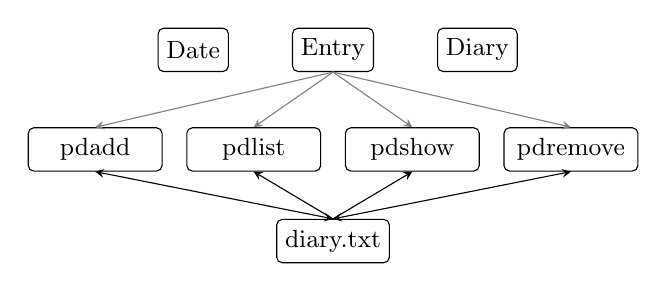
\begin{tikzpicture}[
    box/.style={draw, rounded corners=2pt, minimum height=5.5mm, inner sep=3pt, font=\small},
    prog/.style={box, minimum width=17mm},
    arr/.style={->, >=stealth},
    node distance=4mm and 3mm]
  \node[prog] (add) {pdadd};
  \node[prog, right=of add]  (list)   {pdlist};
  \node[prog, right=of list] (show)   {pdshow};
  \node[prog, right=of show] (remove) {pdremove};

  \coordinate (mid) at ($(list.north)!0.5!(show.north)$);
  \node[box, above=7mm of mid] (entry) {Entry};
  \node[box, left=8mm of entry] (date) {Date};
  \node[box, right=8mm of entry] (diary) {Diary};

  \foreach \p in {add, list, show, remove}
    \draw[arr, gray] (entry.south) -- (\p.north);

  \node[box, below=6mm of $(list.south)!0.5!(show.south)$] (file) {diary.txt};
  \foreach \p in {add, remove}
    \draw[arr, <->] (\p.south) -- (file.north);
  \foreach \p in {list, show}
    \draw[arr, <-] (\p.south) -- (file.north);
\end{tikzpicture}
\end{center}

\section{Testing}

Each program is compiled with Date.cpp and Diary.cpp, as described in
README.md. pd.sh runs a program by its name, for example
\texttt{bash pd.sh pdshow 20261105}.

\texttt{bash pd.sh test} tests adding, listing, replacing, redirection and
pipes, removing, and wrong input in a temporary directory. All tests passed.

\section{Problems}

At first parse was a normal member function, so Date::parse could not be called
without an object. I made it static.

pdremove returns $-1$, but the shell shows 255, so the test checks for 255.

At first pdshow and pdlist also saved the file. In a pipe like
\texttt{pdshow A | pdadd B}, both programs run at the same time, and entries
were sometimes lost. Now they do not save the file.

\section{Conclusion}

The programs can add, list, show and remove diary entries, and work together
through redirection, pipes and pd.sh. Build and run instructions are in
README.md.

\end{document}
